% title: Capture or replace a checkpointed value
% description: The producer still runs. Collect captures its checkpointed value; inject replaces the value passed to downstream equations.
\documentclass[tikz,border=5pt]{standalone}
\usetikzlibrary{arrows.meta,calc,shapes.geometric}
\definecolor{numeric}{HTML}{4477AA}
\definecolor{textual}{HTML}{AA4499}

\tikzset{
    box/.style={draw, line width=0.8pt, minimum height=0.8cm,
                minimum width=1.8cm, inner sep=6pt, align=center},
    ir/.style={box},
    flow/.style={-{Stealth[length=5pt]}, line width=0.9pt},
    feedback/.style={flow, dashed},
    note/.style={font=\small, align=center},
    choice/.style={diamond, draw, line width=0.8pt,
                   aspect=2, inner sep=2pt, align=center},
}

\newcommand{\irframe}[2]{
    \draw[line width=0.8pt] #1 rectangle #2;
}

\newcommand{\transformarrow}[4][above]{
    \draw[flow] (#2) -- node[#1=6pt,note] {#4} (#3);
}

\begin{document}
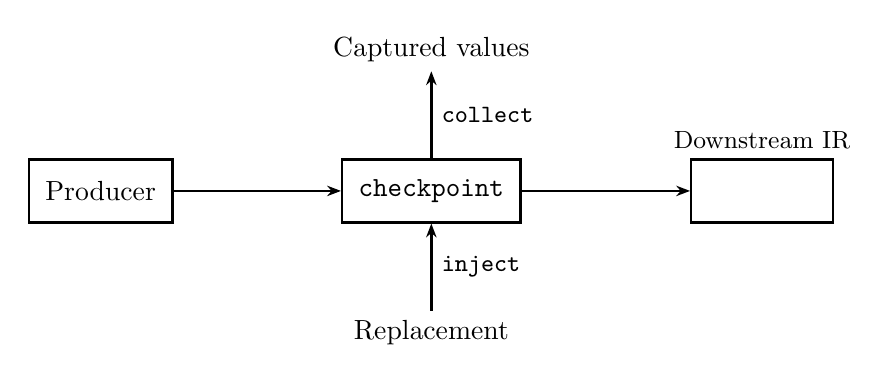
\begin{tikzpicture}

    \node[box] (producer) at (0,0) {Producer};
    \node[box] (checkpoint) at (4.2,0) {\texttt{checkpoint}};
    \node[ir, label={[note]above:Downstream IR}] (downstream) at (8.4,0) {};
    \node[align=center] (captured) at (4.2,1.8) {Captured values};
    \node[align=center] (replacement) at (4.2,-1.8) {Replacement};
    \draw[flow] (producer) -- (checkpoint);
    \draw[flow] (checkpoint) -- (downstream);
    \draw[flow] (checkpoint) -- node[right,note] {\texttt{collect}} (captured);
    \draw[flow] (replacement) -- node[right,note] {\texttt{inject}} (checkpoint);

\end{tikzpicture}
\end{document}
